\documentclass{standalone}
\usepackage{tikz}
\usetikzlibrary{patterns, positioning}

\begin{document}
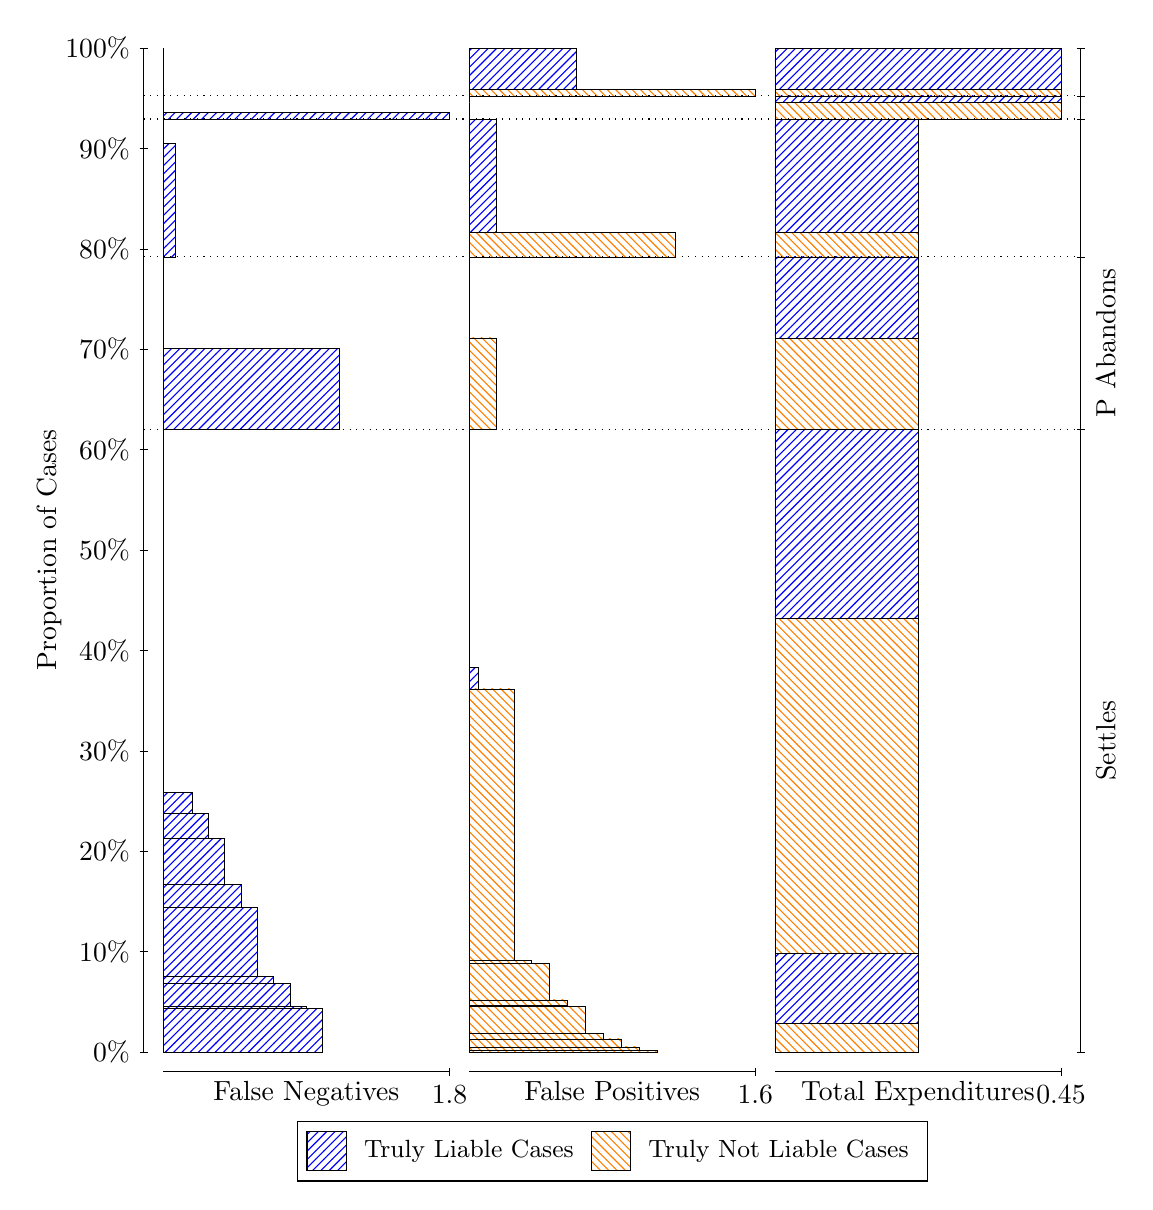
\begin{tikzpicture}
\draw[black, very thin] (1.5,1.75) -- (1.5,14.5);
\node[rotate=90, anchor=center] at (0.3, 8.125) {Proportion of Cases};
\draw[black, very thin] (1.45,1.75) -- (1.55,1.75);
\node[anchor=east] at (1.45, 1.75) {0\%};
\draw[black, very thin] (1.45,3.025) -- (1.55,3.025);
\node[anchor=east] at (1.45, 3.025) {10\%};
\draw[black, very thin] (1.45,4.3) -- (1.55,4.3);
\node[anchor=east] at (1.45, 4.3) {20\%};
\draw[black, very thin] (1.45,5.575) -- (1.55,5.575);
\node[anchor=east] at (1.45, 5.575) {30\%};
\draw[black, very thin] (1.45,6.85) -- (1.55,6.85);
\node[anchor=east] at (1.45, 6.85) {40\%};
\draw[black, very thin] (1.45,8.125) -- (1.55,8.125);
\node[anchor=east] at (1.45, 8.125) {50\%};
\draw[black, very thin] (1.45,9.4) -- (1.55,9.4);
\node[anchor=east] at (1.45, 9.4) {60\%};
\draw[black, very thin] (1.45,10.675) -- (1.55,10.675);
\node[anchor=east] at (1.45, 10.675) {70\%};
\draw[black, very thin] (1.45,11.95) -- (1.55,11.95);
\node[anchor=east] at (1.45, 11.95) {80\%};
\draw[black, very thin] (1.45,13.225) -- (1.55,13.225);
\node[anchor=east] at (1.45, 13.225) {90\%};
\draw[black, very thin] (1.45,14.5) -- (1.55,14.5);
\node[anchor=east] at (1.45, 14.5) {100\%};

\draw[black, very thin] (13.4,1.75) -- (13.4,14.5);
\draw[black, very thin] (13.35,1.75) -- (13.45,1.75);
\node[anchor=west] at (13.35, 1.75) {};
\draw[black, very thin] (13.35,9.6591) -- (13.45,9.6591);
\node[anchor=west] at (13.35, 9.6591) {};
\draw[black, very thin] (13.35,11.847) -- (13.45,11.847);
\node[anchor=west] at (13.35, 11.847) {};
\draw[black, very thin] (13.35,13.598) -- (13.45,13.598);
\node[anchor=west] at (13.35, 13.598) {};
\draw[black, very thin] (13.35,13.892) -- (13.45,13.892);
\node[anchor=west] at (13.35, 13.892) {};
\draw[black, very thin] (13.35,14.5) -- (13.45,14.5);
\node[anchor=west] at (13.35, 14.5) {};

\draw[black, very thin, pattern color=blue, pattern=north east lines] (1.75,1.75) rectangle (3.7743,2.2997);
\draw[black, very thin, pattern color=blue, pattern=north east lines] (1.75,2.2997) rectangle (3.5667,2.3316);
\draw[black, very thin, pattern color=blue, pattern=north east lines] (1.75,2.3316) rectangle (3.359,2.6195);
\draw[black, very thin, pattern color=blue, pattern=north east lines] (1.75,2.6195) rectangle (3.1514,2.7085);
\draw[black, very thin, pattern color=blue, pattern=north east lines] (1.75,2.7085) rectangle (2.9438,3.5851);
\draw[black, very thin, pattern color=blue, pattern=north east lines] (1.75,3.5851) rectangle (2.7362,3.8782);
\draw[black, very thin, pattern color=blue, pattern=north east lines] (1.75,3.8782) rectangle (2.5286,4.4649);
\draw[black, very thin, pattern color=blue, pattern=north east lines] (1.75,4.4649) rectangle (2.321,4.7775);
\draw[black, very thin, pattern color=blue, pattern=north east lines] (1.75,4.7775) rectangle (2.1133,5.0471);
\draw[black, very thin, pattern color=orange, pattern=north west lines] (1.75,5.0471) rectangle (1.75,9.6591);
\draw[black, very thin, pattern color=blue, pattern=north east lines] (1.75,9.6591) rectangle (3.9819,10.688);
\draw[black, very thin, pattern color=orange, pattern=north west lines] (1.75,10.688) rectangle (1.75,11.847);
\draw[black, very thin, pattern color=blue, pattern=north east lines] (1.75,11.847) rectangle (1.9057,13.289);
\draw[black, very thin, pattern color=orange, pattern=north west lines] (1.75,13.289) rectangle (1.75,13.598);
\draw[black, very thin, pattern color=blue, pattern=north east lines] (1.75,13.598) rectangle (5.3833,13.684);
\draw[black, very thin, pattern color=orange, pattern=north west lines] (1.75,13.684) rectangle (1.75,13.892);
\draw[black, very thin, pattern color=orange, pattern=north west lines] (1.75,13.892) rectangle (1.75,13.979);
\draw[black, very thin, pattern color=blue, pattern=north east lines] (1.75,13.979) rectangle (1.75,14.5);
\draw[black, very thin, pattern color=orange, pattern=north west lines] (5.6333,1.75) rectangle (8.0177,1.7729);
\draw[black, very thin, pattern color=orange, pattern=north west lines] (5.6333,1.7729) rectangle (7.7906,1.8136);
\draw[black, very thin, pattern color=orange, pattern=north west lines] (5.6333,1.8136) rectangle (7.5635,1.9156);
\draw[black, very thin, pattern color=orange, pattern=north west lines] (5.6333,1.9156) rectangle (7.3365,1.9838);
\draw[black, very thin, pattern color=orange, pattern=north west lines] (5.6333,1.9838) rectangle (7.1094,2.3296);
\draw[black, very thin, pattern color=orange, pattern=north west lines] (5.6333,2.3296) rectangle (6.8823,2.3423);
\draw[black, very thin, pattern color=orange, pattern=north west lines] (5.6333,2.3423) rectangle (6.8823,2.4104);
\draw[black, very thin, pattern color=orange, pattern=north west lines] (5.6333,2.4104) rectangle (6.6552,2.8787);
\draw[black, very thin, pattern color=orange, pattern=north west lines] (5.6333,2.8787) rectangle (6.4281,2.916);
\draw[black, very thin, pattern color=orange, pattern=north west lines] (5.6333,2.916) rectangle (6.201,6.362);
\draw[black, very thin, pattern color=blue, pattern=north east lines] (5.6333,6.362) rectangle (5.7469,6.6316);
\draw[black, very thin, pattern color=blue, pattern=north east lines] (5.6333,6.6316) rectangle (5.6333,9.6591);
\draw[black, very thin, pattern color=orange, pattern=north west lines] (5.6333,9.6591) rectangle (5.974,10.818);
\draw[black, very thin, pattern color=blue, pattern=north east lines] (5.6333,10.818) rectangle (5.6333,11.847);
\draw[black, very thin, pattern color=orange, pattern=north west lines] (5.6333,11.847) rectangle (8.2448,12.156);
\draw[black, very thin, pattern color=blue, pattern=north east lines] (5.6333,12.156) rectangle (5.974,13.598);
\draw[black, very thin, pattern color=orange, pattern=north west lines] (5.6333,13.598) rectangle (5.6333,13.806);
\draw[black, very thin, pattern color=blue, pattern=north east lines] (5.6333,13.806) rectangle (5.6333,13.892);
\draw[black, very thin, pattern color=orange, pattern=north west lines] (5.6333,13.892) rectangle (9.2667,13.979);
\draw[black, very thin, pattern color=blue, pattern=north east lines] (5.6333,13.979) rectangle (6.9958,14.5);
\draw[black, very thin, pattern color=orange, pattern=north west lines] (9.5167,1.75) rectangle (11.333,2.1084);
\draw[black, very thin, pattern color=blue, pattern=north east lines] (9.5167,2.1084) rectangle (11.333,3.0017);
\draw[black, very thin, pattern color=orange, pattern=north west lines] (9.5167,3.0017) rectangle (11.333,7.2553);
\draw[black, very thin, pattern color=blue, pattern=north east lines] (9.5167,7.2553) rectangle (11.333,9.6591);
\draw[black, very thin, pattern color=orange, pattern=north west lines] (9.5167,9.6591) rectangle (11.333,10.818);
\draw[black, very thin, pattern color=blue, pattern=north east lines] (9.5167,10.818) rectangle (11.333,11.847);
\draw[black, very thin, pattern color=orange, pattern=north west lines] (9.5167,11.847) rectangle (11.333,12.156);
\draw[black, very thin, pattern color=blue, pattern=north east lines] (9.5167,12.156) rectangle (11.333,13.598);
\draw[black, very thin, pattern color=orange, pattern=north west lines] (9.5167,13.598) rectangle (13.15,13.806);
\draw[black, very thin, pattern color=blue, pattern=north east lines] (9.5167,13.806) rectangle (13.15,13.892);
\draw[black, very thin, pattern color=orange, pattern=north west lines] (9.5167,13.892) rectangle (13.15,13.979);
\draw[black, very thin, pattern color=blue, pattern=north east lines] (9.5167,13.979) rectangle (13.15,14.5);
\draw[black, dotted] (1.5,9.6591) -- (13.4,9.6591);
\draw[black, dotted] (1.5,11.847) -- (13.4,11.847);
\draw[black, dotted] (1.5,13.598) -- (13.4,13.598);
\draw[black, dotted] (1.5,13.892) -- (13.4,13.892);
\draw[black, very thin] (1.75,1.5) -- (5.3833,1.5);
\node[anchor=north] at (3.5667, 1.5) {False Negatives};
\draw[black, very thin] (5.3833,1.45) -- (5.3833,1.55);
\node[anchor=north] at (5.3833, 1.45) {1.8};

\draw[black, very thin] (5.6333,1.5) -- (9.2667,1.5);
\node[anchor=north] at (7.45, 1.5) {False Positives};
\draw[black, very thin] (9.2667,1.45) -- (9.2667,1.55);
\node[anchor=north] at (9.2667, 1.45) {1.6};

\draw[black, very thin] (9.5167,1.5) -- (13.15,1.5);
\node[anchor=north] at (11.333, 1.5) {Total Expenditures};
\draw[black, very thin] (13.15,1.45) -- (13.15,1.55);
\node[anchor=north] at (13.15, 1.45) {0.45};

\node[black, centered, rotate=90] at (13.72, 5.7046) {Settles};
\node[black, centered, rotate=90] at (13.72, 10.753) {P Abandons};




\draw (7.449999999999999,1.5) node[draw=none] (baseCoordinate) {};
\begin{scope}[align=center]
        \matrix[scale=0.5, draw=black, below=0.5cm of baseCoordinate, nodes={draw}, column sep=0.1cm]{
            \node[rectangle, draw, minimum width=0.5cm, minimum height=0.5cm, pattern=north east lines, pattern color=blue] {}; &
            \node[draw=none, font=\small] (B) {Truly Liable Cases}; &
            \node[rectangle, draw, minimum width=0.5cm, minimum height=0.5cm, pattern=north west lines, pattern color=orange] {}; &
            \node[draw=none, font=\small] (B) {Truly Not Liable Cases}; \\
            };
\end{scope}

\end{tikzpicture}
\end{document}